\subsection{Architectural styles and patterns}

Apps are as of today on nearly all platforms primarily developed in an object-oriented style. This only seems natural as "the benefits of OOP include encapsulation mechanisms and intuitive ways to model complex domains in software. OOP is a natural fit for GUIs, which probably drove the mainstream adoption of OOP in the 1980s, when GUIs also went mainstream. Once prevalent, OOP also proved broadly applicable." (\cite{wampler_guest_2010}).

Closely attached to OOP are five principles that shall enable developers to build understandable, flexible, and maintainable software: "The SOLID principles are a set of basic principles for designing OO programs. The name itself is an acronym, with each of the five principles named after one of the letters: Single responsibility, Open/ closed, Liskov substitution, Interface segregation, and Dependency inversion. The principles act as a set of guidelines to help you implement code that is easy to maintain and extend over time." (\cite[7]{warburton_object-oriented_2016}).

Apart from those fundamental principles, patterns often arise around specific tasks. At some point, they are then (formally) described and given a name. The original design pattern that many developers apply when building native iOS and Android apps is Model-View-Controller (MVC). It was presumably first described by \cite{krasner_description_1988} and has been the starting point for experiments and the discovery of many derived architectural styles since. A lot of different patterns have been proposed for building mobile applications in particular, e.g., VIPER (\cite{gilbert_architecting_2014}), Clean Swift (\cite{law_clean_2015}), or MVI (\cite{dorfmann_model-view-intent_2016}).

\begin{figure}[H]
\centering
\caption{The MVVM Architectural Pattern}
\label{fig:chasm}
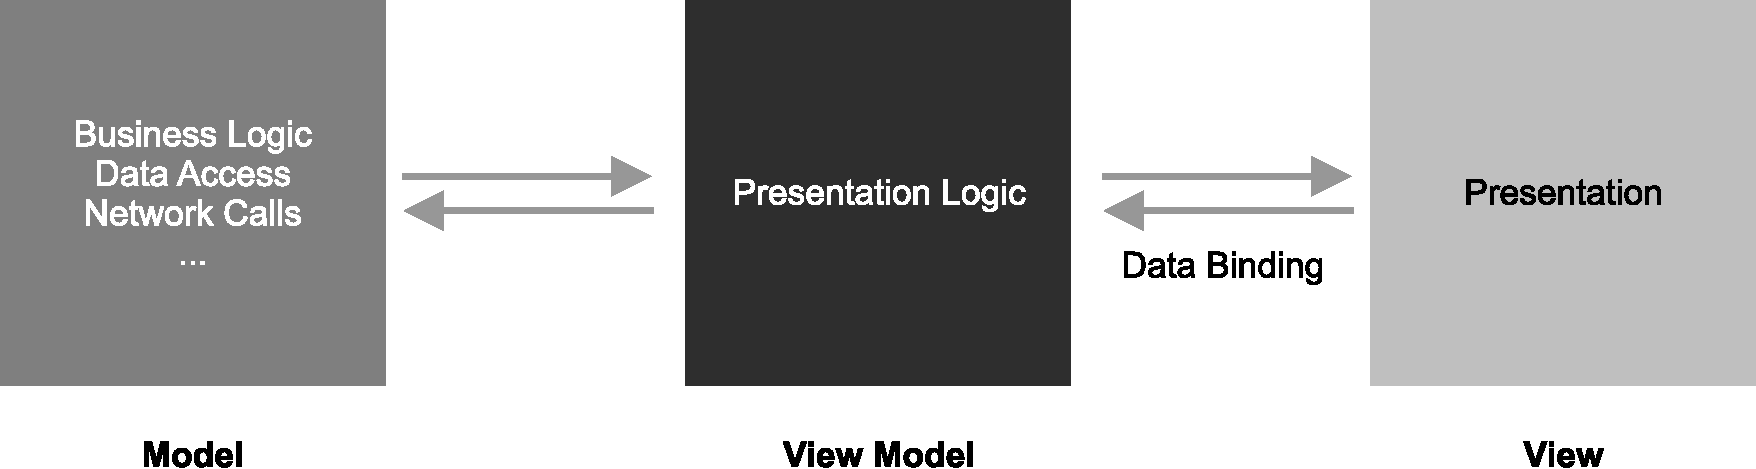
\includegraphics[width=\textwidth]{mvvm}
\source{Own illustration}
\end{figure}

However, the dominating pattern used for building Xamarin apps is Model-View-View Model (MVVM). First mentioned by \cite{gossman_introduction_2005} in the context of Windows desktop development, it made its way to mobile app development later on. Xamarin made the transition especially easy for developers used to technologies like WPF, where MVVM was already successfully applied, by supporting it natively with Xamarin.Forms. But also for Xamarin.iOS and Xamarin.Android developers can chose from a wide range of MVVM frameworks and libraries like MvvmCross\footnote{https://www.mvvmcross.com/ (retrieved August 8, 2019)}, ReactiveUI\footnote{https://reactiveui.net/ (retrieved August 8, 2019)}, or Prism\footnote{https://prismlibrary.github.io/docs/ (retrieved August 8, 2019)}.
